\chapter{Teamwork}
\section{Reflection}
Because of the design of the application many parts can be developed at the same time, especially cause we used Unit Tests for the Data and Business layer. We used Git for the documentation and code, it went very well for the documentation since we used \LaTeX so we could work on the same document and not worry about losing data. Our communication went smoothly through a chatting program and working together in school. For the decision making we did not argue much and decisions were made rather quickly. The progress of the application went very evenly and we always hand it in before the deadlines we had in mind. One person might spent too much effort in the Quality Assurance of the project. But that became much less the more we worked on it which is very noticeable in the Presentation Layer which contains a \emph{huge} god class \texttt{MainWindow}. It should be refactored in many more smaller classes and follow the SOLID principals, and the view of the MainWindow could have had much more responsibility.

\chapter{Working method}
\section{Iterative working}
We wished to work in a more iterative way, like each week review a new chapter of a document. Take for example the design document, where we could have spend a lot of time refactoring the class diagram and sequence diagrams if the system overview was not agreed on. In the beginning we didn't had very clear agreements on when the deadline exactly was. And didn't get much feedback. One person in the group really want this done to study for the exams, in return we get the deadline the next morning. Then we aren't really waiting for the feedback on the documents since there is not much time to update it. This does not feel like our responsibility to step in and change the design of the course, clearly there should be 2 hours scheduled in on Monday morning for the teachers to review the deliverables so everyone has a fair deadline in the weekend.

\section{Waterfall or Agile}
Many might argue that working more iterative is Agile. Let's look at the definition of agile in figure \ref{fig:agile}. Notice that the word has been misused all the time! It is an adjective, why would you even write it with a capital letter. So you can say working more iterative is more like an Agile working method. What happens when you work with such a working method like SCRUM, the customer can have many more crazy ideas just at the end and there is nothing what you can do about. And when something isn't like the customer likes the developer has no feet to stand on unlike showing some documentation. Ok we skipped some features in the hope we didn't had too implement them but we knew that we agreed upon that design and had to implement it anyway. It shows that using waterfall working method is much better to use with a bad cooperating customer. It is weird to see that when you work really hard all your life and you end up here. In a bachelor degree in a so called civilized and developed country. For which you have to pay an arm and a leg to go to. And seems like the most things they teach are complete \emph{bullshit}. They totally felled for the Agile and SCRUM marketing, instead of keeping up with the latest information. Please let the coming 'Agile' project not be disappointing. I almost seem to believe that SCRUM is created by the waterfall people to get rid of Agile forever.

\begin{figure}[h!]
	\centering
	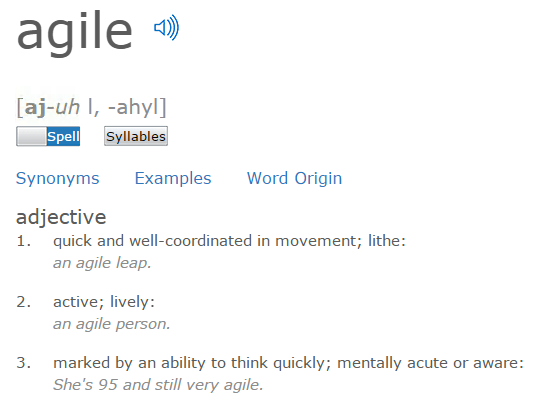
\includegraphics[width=\textwidth]{agile.png}
	\caption{Definition of agile.}
	\label{fig:agile}
\end{figure}


  

\begin{sidewaystable}[]
	\centering
	\begin{tabular}{lllllllllll}
		\textbf{Scope}  & \textbf{Activity}  & \textbf{Responsible} & \textbf{WK1} & \textbf{WK2} & \textbf{WK3} & \textbf{WK4} & \textbf{WK5} & \textbf{H1} & \textbf{H2} & \textbf{WK6} \\
		Process report  & Work breakdown     & All                  &              & 2            & 1            &              & 0,5          & 0,5         &             & 0,5          \\
		URS             & Requirements       & Wen                  & 1            &              &              &              &              & 0,5         &             &              \\
		URS             & Use cases          & Edgar                & 3            & 2            & 1            &              &              &             &             & 0,5          \\
		URS             & Use cases          & Wen                  & 3            & 2            & 1            &              &              &             &             &              \\
		URS             & Use cases          & Coen                 & 1            &              &              &              &              & 0,5         &             &              \\
		URS             & UI                 & Wen                  &              & 3            & 0,5          &              &              & 0,5         &             & 0,5          \\
		URS             & UI specifications  & Wen                  &              & 1            & 0,5          &              &              & 0,5         &             &              \\
		URS             & Non-functional     & Wen                  &              & 2            &              &              &              &             &             &              \\
		Design document & Introduction       & Coen                 &              & 3            &              &              &              &             &             &              \\
		Design document & Class diagram      & Coen                 &              &              & 3            & 0,5          &              & 1           &             &              \\
		Design document & Sequence diagrams  & Coen                 &              &              &              & 4            &              & 1           &             &              \\
		Implementation  & Create project     & Coen                 &              &              &              &              & 0,5          &             &             &              \\
		Implementation  & Common layer       & Edgar                &              &              &              &              & 2            & 0,5         &             &              \\
		Implementation  & Business layer     & Wen                  &              &              &              &              & 5            & 6           &             &              \\
		Implementation  & Business layer     & Coen                 &              &              &              &              & 2            & 2           &             &              \\
		Implementation  & Data layer         & Edgar                &              &              &              &              & 1            & 3           &             &              \\
		Implementation  & Data layer         & Coen                 &              &              &              &              &              & 3           &             &              \\
		Implementation  & Launcher           & Coen                 &              &              &              &              &              & 0,5         &             &              \\
		Implementation  & Presentation layer & Wen                  &              &              &              &              & 1            & 7           &             &              \\
		Implementation  & Presentation layer & Edgar                &              &              &              &              &              & 10          &             &              \\
		Implementation  & Presentation layer & Coen                 &              &              &              &              &              & 4           &             & 4            \\
		Process report  & Discussion         & Coen                 &              &              &              &              &              &             &             & 3           
	\end{tabular}
\end{sidewaystable}